\begin{figure}[h]
	\centering
	
	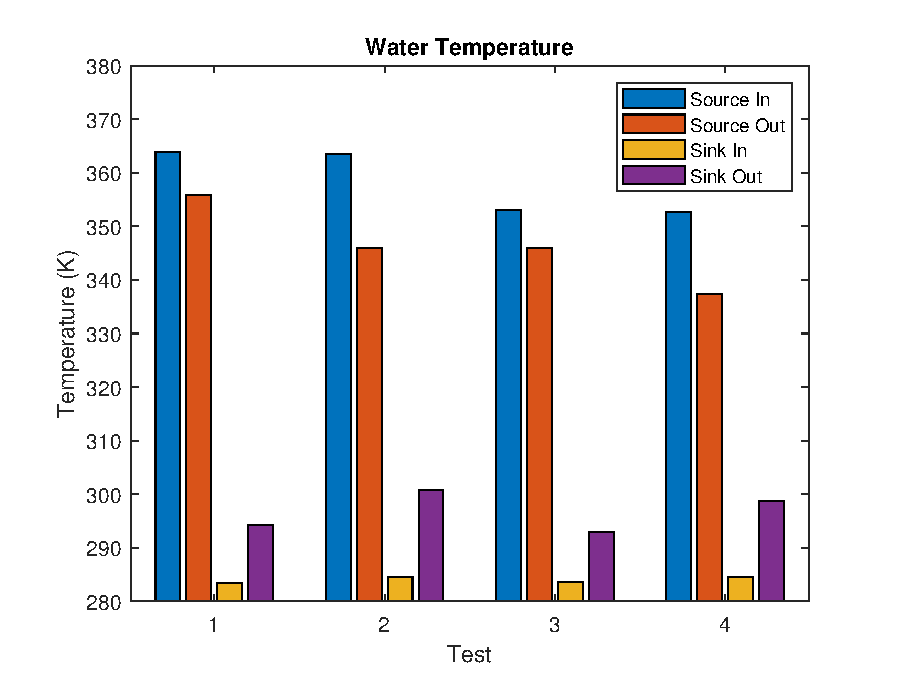
\includegraphics[width=\textwidth]{figures/VerificationWaterTemp01}
	%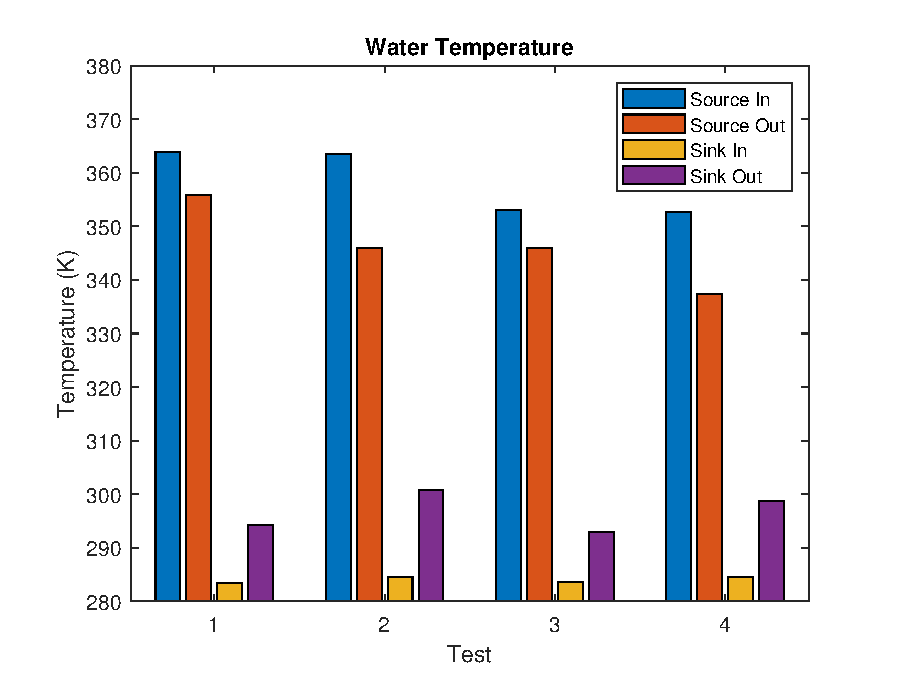
\includegraphics[width=0.5\textwidth]{figures/VerificationWaterTemp01}
	
	\caption{Comparison of source and sink inlet and outlet temperatures for the validation of the ORC prime power system model. All tests assume a sink temperature of \SI{283}{\kelvin} (\SI{10}{\degreeCelsius}). Tests 1 \& 2 use a heat source temperature of \SI{364}{\kelvin} (\SI{91}{\degreeCelsius}), while tests 3 \& 4 use \SI{353}{\kelvin} (\SI{79}{\degreeCelsius}). Tests 1 \& 3 use a source flow rate of \SI{19}{\liter\per\second} and a sink flow rate of \SI{13}{\liter\per\second}, where as test 3 \& 4 use a source and sink flow rate of \SI{8}{\liter\per\second}.
	%The power setpoints of the four tests are \SIlist{27.5;40.0;30.8;42.0}{\kilo\watt}. Tests 1 \& 3 use the maximum power setpoint while also ensuring the working fluid fully evaporates in the evaporator. Tests 2 \& 4, use the maximum power setpoint while maintaining a stable simulation. 
	}
	%Psetpoint[2.75e4;4.0e4;3.08e4;4.2e4;]
	\label{fig:verificationWaterTemp01}
\end{figure}